\documentclass[a4paper]{article}
\usepackage[a4paper, margin=1.5cm]{geometry}
%\usepackage[francais]{babel}
\usepackage[T1]{fontenc}
\usepackage[utf8]{inputenc}
\usepackage{graphicx}
\usepackage{xcolor}
\usepackage{tcolorbox}
\usepackage{url}
\usepackage{tikz}
\usetikzlibrary{shapes.geometric, arrows.meta, positioning, shadows, calc}

% Standardized Colors
\definecolor{lokadblue}{HTML}{005696}
\definecolor{xgreen}{HTML}{006633}
\definecolor{boxfill}{HTML}{D9EFFF}
\definecolor{boxstroke}{HTML}{58B9EF}
\definecolor{arrowcolor}{HTML}{1F2937}

\newcommand{\labelstyle}[1]{{\scriptsize\normalfont\color{gray!80!black} #1}}

\begin{document}
\pagenumbering{gobble}

% Header with logos
\noindent
\begin{minipage}{0.3\textwidth}
    
\includegraphics[height=1.4cm]{../assets/x.pdf}
\end{minipage}
\begin{minipage}{0.4\textwidth}
    \centering
    \small \textbf{École Polytechnique - PSC X24} \\
    \small \textsc{Page publique}
\end{minipage}
\begin{minipage}{0.3\textwidth}
    \flushright
    
\includegraphics[height=1.4cm]{../assets/lokad.png}
\end{minipage}

\vspace{0.8cm}

\begin{center}
    {\Huge \bfseries \color{lokadblue} PSC INF01} \\[0.3cm]
    {\Large \itshape Architecture Agentique et Hybride pour l'Extraction de Connaissances sur Code Propriétaire (Envision)}
\end{center}

\vspace{0.6cm}

\begin{tcolorbox}[colback=lokadblue!5!white,colframe=lokadblue,title=\centering \bfseries L'Équipe INF01]
    \centering
    \large \textbf{Gaétan Dégot--Silvestre, Yoan Dorchies, Ivann Kamdem, Guilhem Thébault, Adam Guediche}
\end{tcolorbox}

\vspace{0.3cm}

\begin{center}
    \section*{Pipeline Agentique}
    
    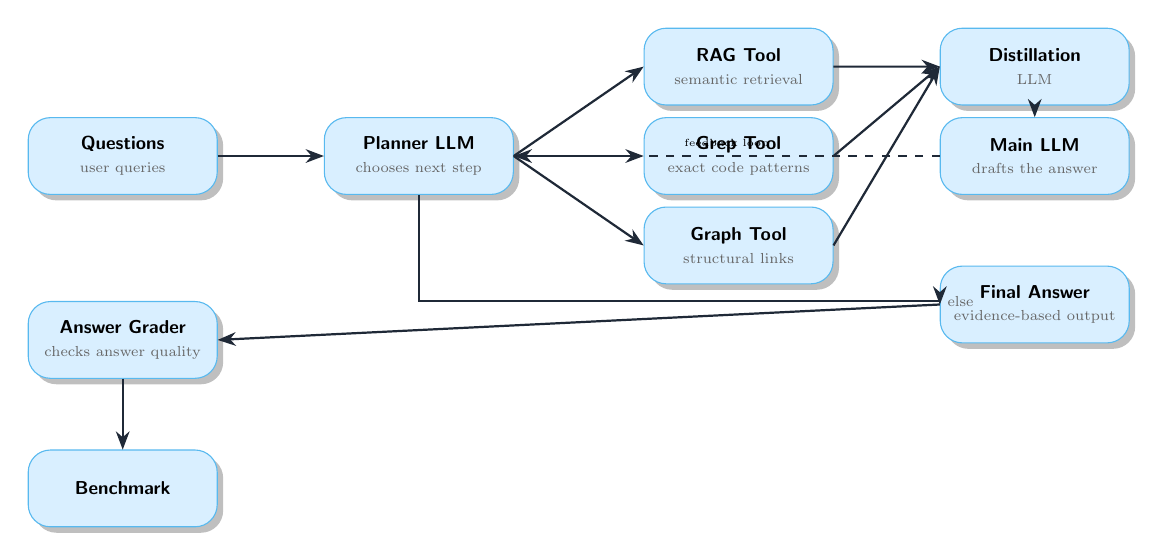
\begin{tikzpicture}[
        scale=0.75, 
        transform shape,
        node distance=1.2cm and 1.8cm,
        box/.style={
            rectangle, 
            rounded corners=8pt, 
            minimum width=3.2cm, 
            minimum height=1.3cm, 
            draw=boxstroke, 
            fill=boxfill, 
            align=center, 
            font=\sffamily\bfseries\small,
            drop shadow
        },
        arrow/.style={-Stealth, thick, draw=arrowcolor}
    ]
        % Nodes
        \node[box] (questions) {Questions \\ \labelstyle{user queries}};
        \node[box, right=of questions] (planner) {Planner LLM \\ \labelstyle{chooses next step}};
        
        % Tools
        \node[box, above right=0.2cm and 2.2cm of planner] (rag) {RAG Tool \\ \labelstyle{semantic retrieval}};
        \node[box, right=2.2cm of planner] (grep) {Grep Tool \\ \labelstyle{exact code patterns}};
        \node[box, below right=0.2cm and 2.2cm of planner] (graph) {Graph Tool \\ \labelstyle{structural links}};
        
        % Processing
        \node[box, right=1.8cm of rag] (distill) {Distillation \\ \labelstyle{LLM}};
        \node[box, right=1.8cm of grep] (mainllm) {Main LLM \\ \labelstyle{drafts the answer}};
        \node[box, below=1.2cm of mainllm] (final) {Final Answer \\ \labelstyle{evidence-based output}};
        
        \node[box, below=1.8cm of questions] (grader) {Answer Grader \\ \labelstyle{checks answer quality}};
        \node[box, below=1.2cm of grader] (benchmark) {Benchmark};
        
        % Arrows
        \draw[arrow] (questions) -- (planner);
        \draw[arrow] (planner.east) -- (rag.west);
        \draw[arrow] (planner.east) -- (grep.west);
        \draw[arrow] (planner.east) -- (graph.west);
        
        \draw[arrow] (rag.east) -- (distill.west);
        \draw[arrow] (grep.east) -- (distill.west);
        \draw[arrow] (graph.east) -- (distill.west);
        
        \draw[arrow] (distill.south) -- (mainllm.north);
        \draw[arrow] (planner.south) -- ++(0, -1.8) -| (final.west) node[pos=0.5, right] {\labelstyle{else}};
        
        \draw[arrow] (final.west) -- (grader.east);
        \draw[arrow] (grader.south) -- (benchmark.north);

        % Loops
        \draw[arrow, dashed] (mainllm.west) -- node[above, font=\tiny] {feedback loop} (planner.east);
        
    \end{tikzpicture}
\end{center}

\vspace{0.4cm}

\begin{tcolorbox}[colback=white,colframe=lokadblue!40,title=\bfseries Résumé du Projet]
Le projet INF01 propose un assistant intelligent conçu pour l'analyse de code propriétaire écrit en \textbf{Envision} (le DSL de Lokad). Le projet résout l'opacité des bases de code massives en utilisant une architecture agentique capable de :
\begin{itemize}
    \item \textbf{Planifier} des stratégies de recherche multi-étapes dynamiques.
    \item \textbf{Extraire} des informations via RAG, Analyse Statique et Graphes de dépendances.
    \item \textbf{Expliquer} le fonctionnement interne du code avec une source de vérité vérifiable.
\end{itemize}
Cette approche permet une autonomie accrue pour les nouveaux développeurs et une compression de la courbe d'apprentissage sur des outils métier complexes.
\end{tcolorbox}

\vfill
\begin{center}
    \small \color{gray} Accédez à la documentation complète \& au code source : \\
    \small \color{gray} Documentation : \textbf{\url{https://kpihx.github.io/envision-copilot-presentation/}} \\
    \small \color{gray} Code source : \textbf{\url{https://github.com/ClementLokad/llm-DSL-info-extraction}}
\end{center}

\end{document}
